Each \dword{apa} is instrumented with \num{20} %Front End Mother Boards (
\dwords{femb}.
The \dwords{femb} plug into the \dword{apa} CR boards, making the connections from the wires to the charge amplifier circuits as short as possible.
Each \dword{femb} receives signals from \num{40} $U$ wires, \num{40} $V$ wires, and \num{48} $X$ wires.
The baseline \dword{femb} design contains eight \num{16}-channel \dword{fe} (\dword{larasic}) \dwords{asic}, eight \num{16}-channel Cold \dword{adc} \dwords{asic}, and two \dword{coldata} control and communication \dwords{asic} (see Figure~\ref{fig:ce-scheme}).
The \dword{femb} also contains regulators that produce the voltages required by the \dwords{asic} and 
filter those voltages.
The \dword{larasic} inputs are protected by diodes and a series inductor.

\begin{dunefigure}
[The baseline \dword{ce} architecture.]
{fig:ce-scheme}
{The baseline \dword{ce} architecture. The basic unit is the \num{128}-channel \dword{femb}. Note that only one \dword{ce} flange is shown to simplify the illustration. Note that \dword{ssp} stands for \textit{SiPM Signal Processor} (see Chapter~\ref{ch:fdsp-pd}).}
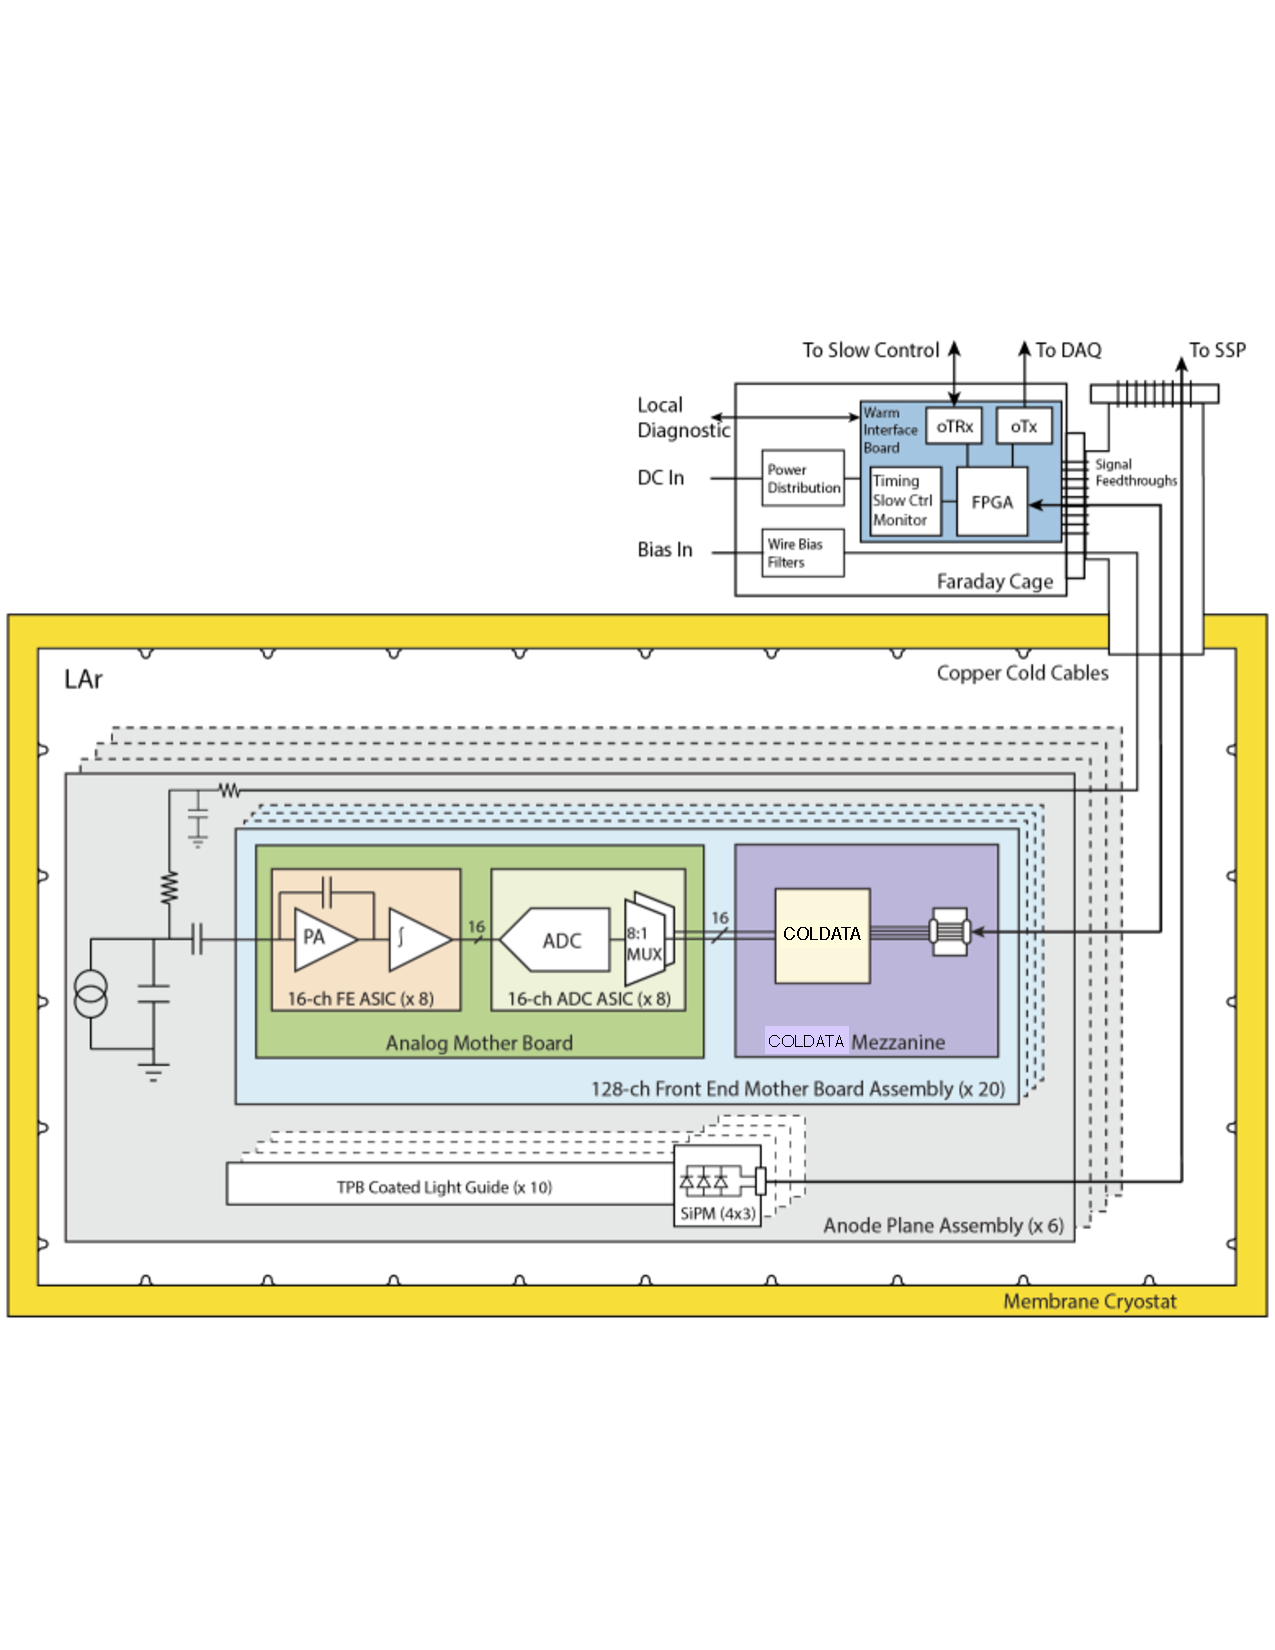
\includegraphics[width=0.9\linewidth]{tpcelec-schem_v2.pdf}
\end{dunefigure}

The \dword{pdsp} version of the \dword{femb} (which uses a single \dword{fpga} on a mezzanine card instead of two \dword{coldata} \dwords{asic}) is shown in Figure~\ref{fig:femb}.

\begin{dunefigure}
[The complete \dword{femb} assembly as used in \dword{pdsp}.]
{fig:femb}
{The complete \dword{femb} assembly as used in the \dword{pdsp} detector. The cable shown is the high-speed data, clock, and control cable.}
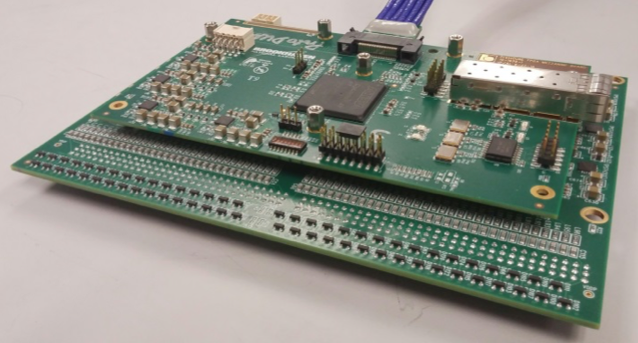
\includegraphics[width=0.6\linewidth]{tpcelec-femb.png}
\end{dunefigure}
